\section{Exploratory Data Analysis}

\begin{frame}{Data Isolation \& Target Distribution}
    \textbf{Strict Data Isolation:}
    \begin{itemize}
        \item Visual analysis strictly limited to the \textbf{Training Set} to prevent \textit{Data Leakage}. Validation and Test sets act as secure "vaults".
    \end{itemize}
    \vspace{0.3cm}
    \textbf{Class Imbalance Check:}
    \begin{itemize}
        \item The dataset is \textbf{sufficiently balanced} (slight natural prevalence of misses).
        \item Eliminates risk of predictive bias; standard metrics (Accuracy) remain reliable.
    \end{itemize}
\end{frame}

\begin{frame}{Spatial Analysis: Kobe Bryant Shot Map}
    \begin{columns}
        \begin{column}{0.4\textwidth}
            \textbf{Key Insights:}
            \begin{itemize}
                \item Mapped using continuous Cartesian coordinates (\texttt{alpha=0.5} to avoid overplotting).
                \item \textbf{Clusters:} High tendency to shoot from the paint and "elbows".
                \item \textbf{Efficiency:} High success near the rim; variance increases with distance.
            \end{itemize}
        \end{column}
        \begin{column}{0.6\textwidth}
            \begin{figure}
                \centering
                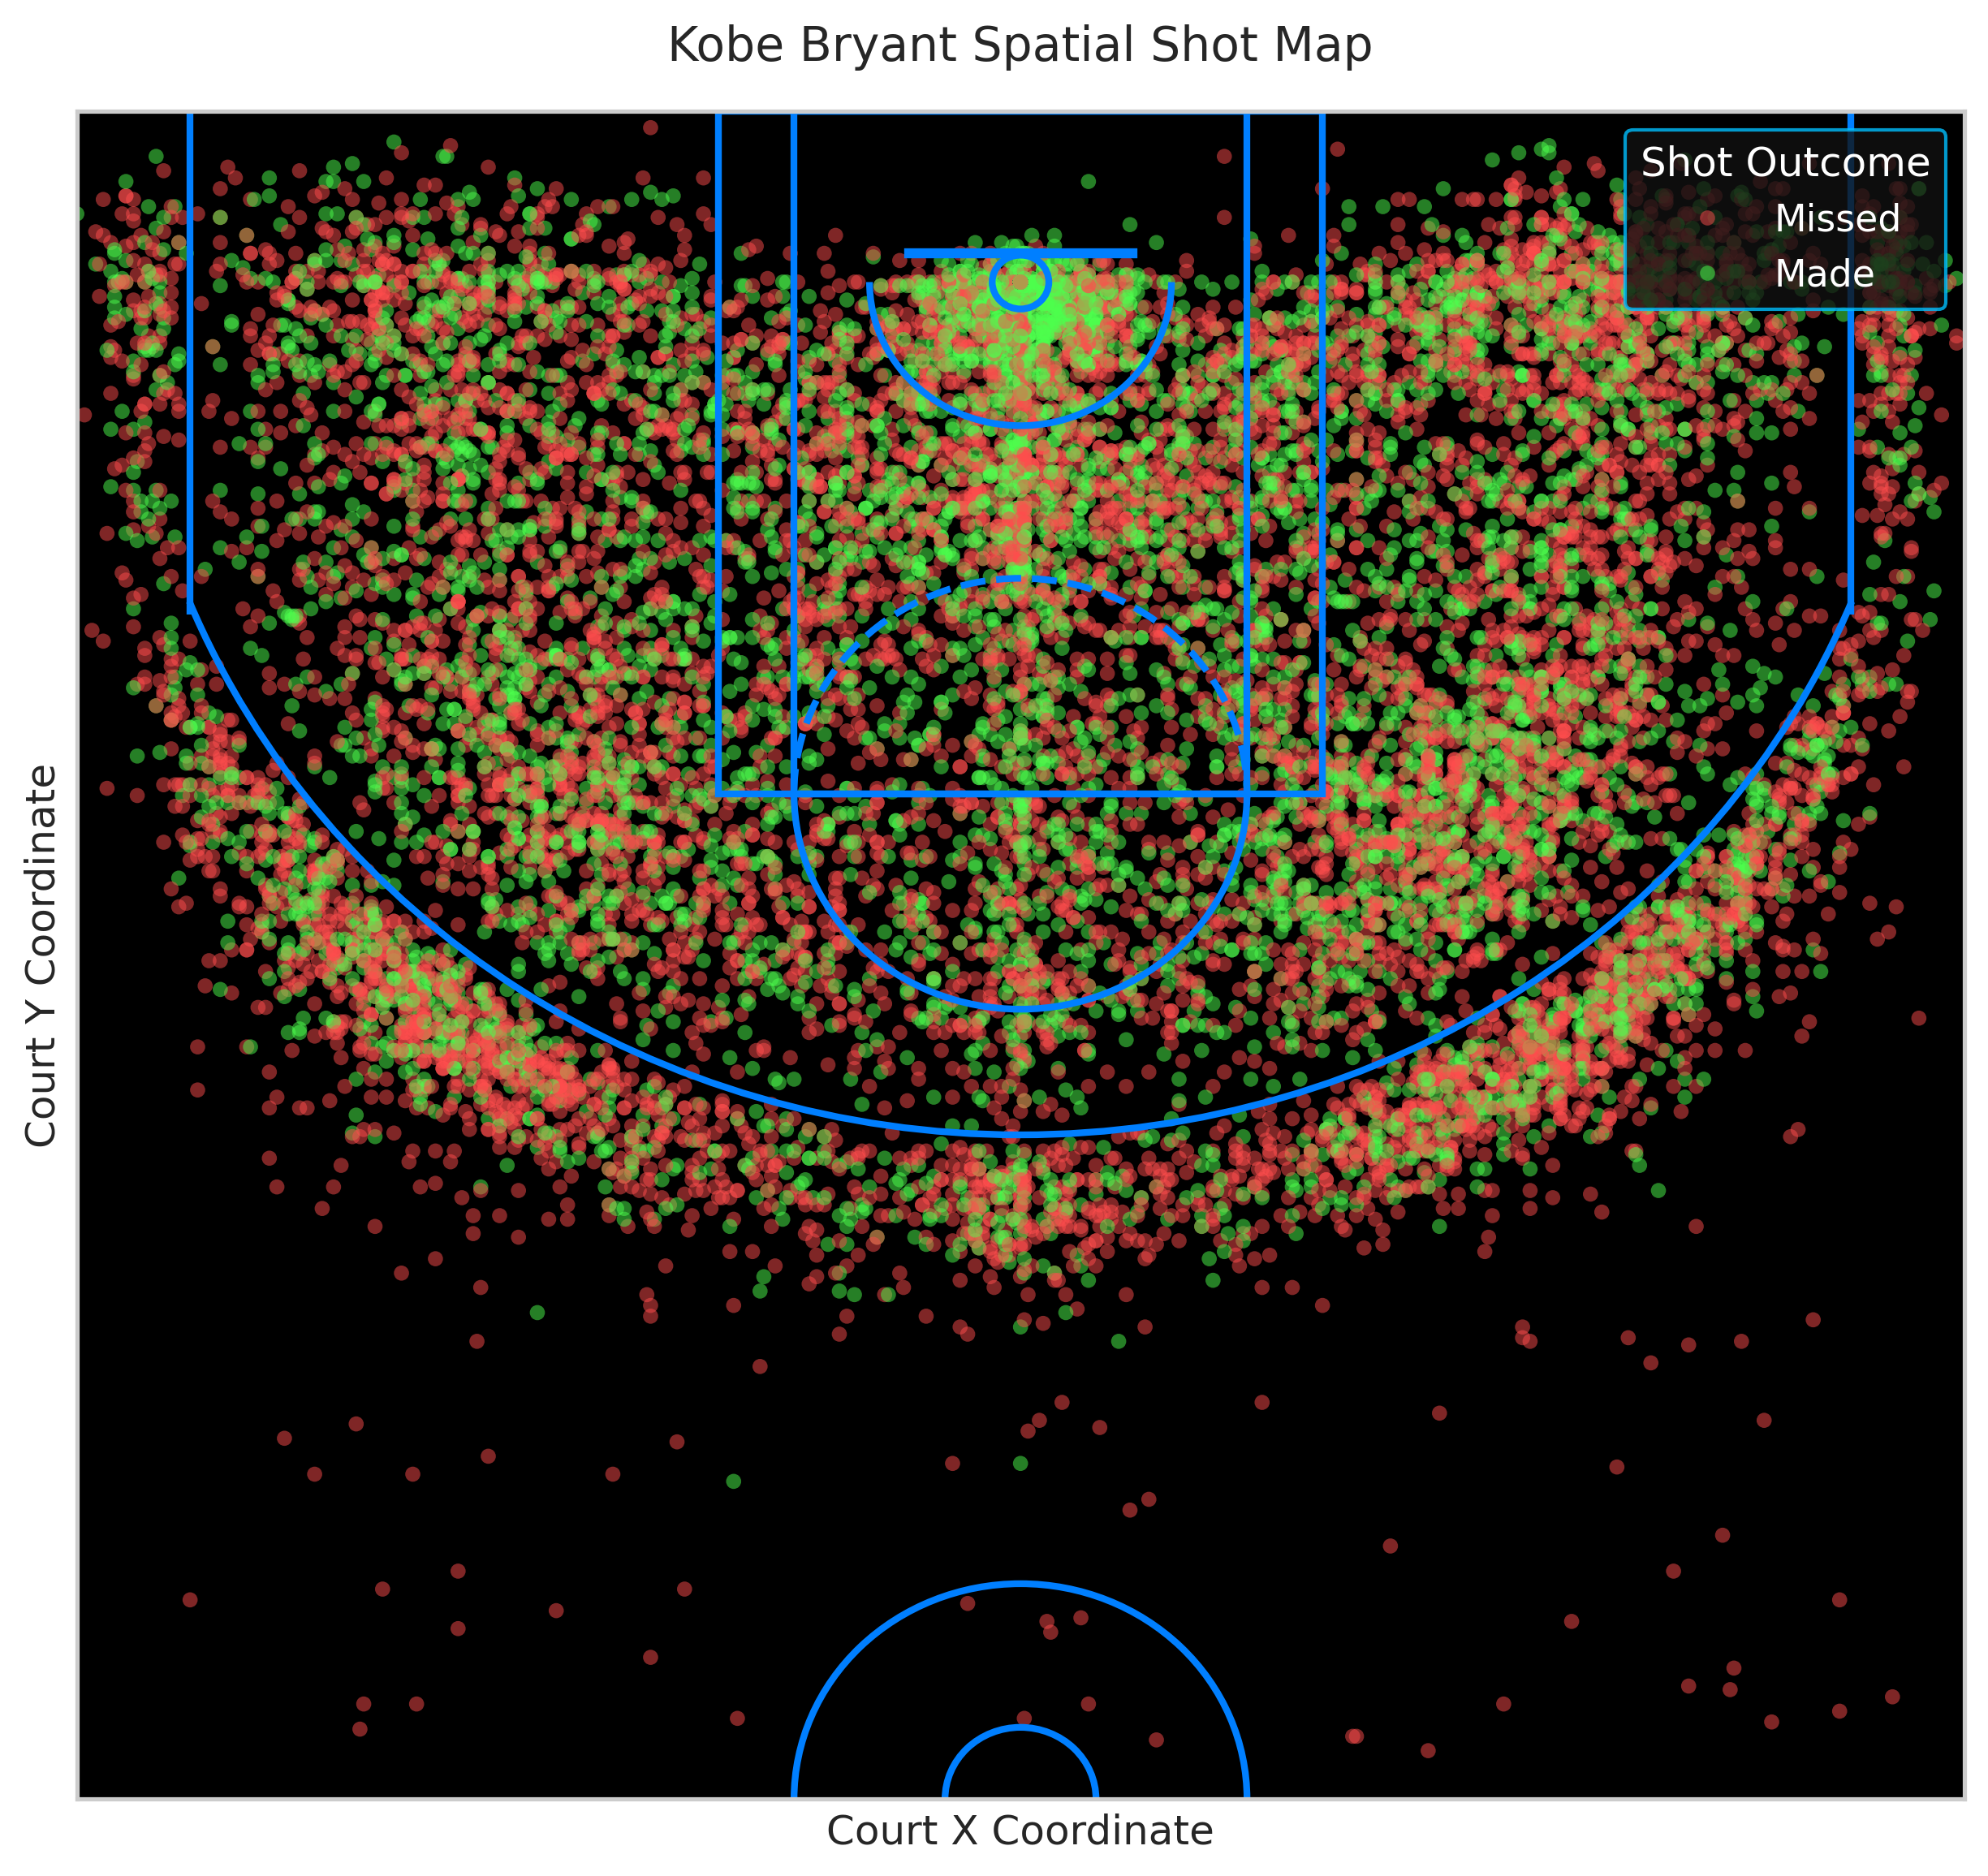
\includegraphics[width=\textwidth]{img/map.png}
            \end{figure}
        \end{column}
    \end{columns}
\end{frame}